% !TEX program = xelatex
% !TEX options = --shell-escape

\documentclass{beamer}

\usepackage[style=numeric,maxnames=2, defernumbers=true]{biblatex}
\usepackage{minted}
\usemintedstyle{colorful}
\usepackage{relsize, xspace}
\usepackage{tikz}
\usepackage{booktabs}
\usepackage{circuitikz}
\usetikzlibrary{shapes}
\usetikzlibrary{shapes.geometric}

\definecolor{lightgray}{gray}{0.9}
\definecolor{arbgrey}{RGB}{84, 84, 84}
\definecolor{arbred}{RGB}{153, 67, 25}
\definecolor{arborange}{RGB}{201, 104, 44}
\definecolor{mediumslateblue}{HTML}{7B68EE}
\newcommand*\circled[1]{\tikz[baseline=(char.base)]{\node[shape=circle,fill,inner sep=2pt] (char) {\textcolor{white}{#1}};}} % chktex 36

\usepackage[orientation=portrait,size=a1,scale=1.0]{beamerposter}
\usetheme{JuelichPoster}

\usetikzlibrary{positioning}

\ExecuteBibliographyOptions{%
  sorting=nyt,
  bibwarn=true,
  isbn=false,
  url=true%
}
\addbibresource{references.bib}

\setbeamertemplate{partner1}{
\includegraphics{img/cscs}}
\setbeamertemplate{partner2}{
\includegraphics{img/HBP_logo}}

\begin{document}

\newcommand{\nmlcc}{\texttt{nmlcc}}
% C++ symbol; picked up from the ISO standard
\newcommand\cpp{C\nolinebreak[4]\hspace{-.05em}\raisebox{.4ex}{\relsize{-3}{\textbf{++}}}}

\begin{frame}[t, fragile]
  \frametitle{
\includegraphics[width=0.66\linewidth]{img/arbor-lines-proto-colour-full}}
  \framesubtitle{Designing a HPC-benchmark for biologically realistic Neuron Simulations\\
    \tiny{T. Hater, B. Huisman (Forschungszentrum Jülich)}}
  \begin{columns}[onlytextwidth,T]
    \begin{column}{0.76\textwidth}
      Computational neuroscience is a major consumer of HPC resources. While
      point models are highly demanding in terms memory and network
      capabilities, networks of morphologically realistic neurons require
      significant computational resources \cite{NEST,arb,nrn}. We present a
      benchmark for studying the performance of such detailed simulations at
      large scales and evaluating HPC-architectures to be used in this setting.
      The basis for this project is Arbor, which has been shown to scale well to
      large nodes counts when using simple cell models \cite{arb}. Here, we
      extend this to a complex model, that is inspired by a model from the Allen
      cell database\cite{allen-v1}. The goal of this project is twofold, first
      to understand and improve the performance of Arbor at scale and second to
      study the suitability of current and emerging HPC architectures for these
      kind of workloads.
    \end{column}
    \begin{column}{0.22\textwidth}
      \vspace*{-1ex}
      \begin{block}{Where to find\dots}
        \begin{description}
          \item[Arbor] \href{https://arbor-sim.github.io}{arbor-sim.github.io}
          \item[Contact] \href{t.hater@fz-juelich.de}{t.hater@fz-juelich.de}
          \item[Poster] \href{https://github.com/thorstenhater/isc-2023}{github.com/thorstenhater/isc-2023}
        \end{description}
      \end{block}
    \end{column}
  \end{columns}
  % problem statement
  \vspace*{1ex}
  \textcolor{arbgrey}{\rule{\textwidth}{0.5ex}}
  \vspace*{-1ex}
  \begin{columns}[t]
    \begin{column}[T]{0.35\textwidth}
      \textbf{Detailed Neuron Models}
      \begin{itemize}
        \item Possess a morphology, split in to compartments
        \item Sub-regions are adorned with active components, i.e.\ ion channels.
        \item Complex neuron behaviour emerges from the interplay of ion
              channels.
        \item Individual ion channels driven by differential equations.
        \item Potential evolution driven by cable equation
              \begin{align*}
                \frac{1}{C_{m}}\partial_{t}U_{m} = \partial_{x}\left(x\partial_{x}\sigma_{l} U_{m}\right) + I_{m}
              \end{align*}
        \item Transmembrane current $I_{m}$ has a leak contribution via $R_{m}$ and a dynamic component for the ion channels.
      \end{itemize}
    \end{column}
    \begin{column}[T]{0.2\textwidth}
      \begin{center}
        \begin{circuitikz}[scale=1.2, every node/.style={transform shape}]
          \draw (0,3.5) to[R=$R_l$] (0,0)
          to[R=$R_l$] (0, -3.5)
          (4,0.5) to [C] (0,0.5)
          to [short]   (0,0)
          (4,0.5) to [short]   (4,0)
          (4,0)   to [short]   (4,-.5)
          to [R] (0,-.5)
          to [short]   (0,0);
          \draw (4,-0.5) -- (4,-1.5) node[ground]{};

          \node[] at (2.5,0.75)  {$C_m$};
          \node[] at (2.5,-0.25) {$R_m$};

          \node[] at (2.5, 1.5) {$I_m$};
          \draw[-stealth] (1.5, 1.2) -- (2.5, 1.2);

          \node[cylinder, ultra thick,
          draw = black!40,
          minimum width = 4cm,
          minimum height = 6cm,
          shape border rotate = 90] (c) at (0,0) {};
        \end{circuitikz}
      \end{center}
    \end{column}
    \begin{column}[T]{0.35\textwidth}
      \textbf{Arbor}
      \begin{itemize}
        \item Performance portable library in \cpp{17} for writing neural network
              simulations.
        \item Accelerator support for NVIDIA and AMD GPUs.
        \item Explicit SIMDisation, custom work-stealing thread-pool, and MPI.
        \item Concurrent communication and computation to hide network
              latencies.
        \item High-level Python interface.
        \item Supports point models and complex cable cells.
        \item Custom DSL compiler for ion channels.
        \item Permissive BSD-3 license
      \end{itemize}
    \end{column}
  \end{columns}

  \vspace*{1ex}
  \textcolor{arbred}{\rule{\textwidth}{0.5ex}}
  \vspace*{-1ex}
  \begin{columns}[t]
    \begin{column}[T]{0.25\textwidth}
      \textbf{The Cell}
      \begin{itemize}
        \item Pseudo-randomly branching tree with tunable
        \begin{itemize}
          \item depth $d$
          \item branching probability $p$
          \item branch lengths $l$
          \item compartments per branch $k$
        \end{itemize}
        \item Two sub-regions with different dynamics
        \item \emph{Soma}
        \begin{itemize}
          \item $6.3\,\mu m$ sphere at the root of the tree
          \item 7 active channels + 1 passive
        \end{itemize}
        \item \emph{Dendrite}
        \begin{itemize}
          \item actual branching structure
          \item 4 active channels + 1 passive
        \end{itemize}
        \item \emph{Synapses} connection are given as simple exponential
              synapses.
        \item Dynamics are based on the Allen Cell database \cite{allen-v1}.
      \end{itemize}
    \end{column}
    \begin{column}[T]{0.45\textwidth}
      \centering
      \begin{tikzpicture}
        \draw[black!40, ultra thick] (0,0) circle(1.5cm);
        \node[regular polygon, regular polygon sides=5, minimum size=3cm] at (0,0) (A) {};
        \foreach \i in {1,...,5}
           \node[circle, fill=black!80] at (A.corner \i) {};
        \draw[black!40, ultra thick] (6,0) circle(1.5cm);
        \node[regular polygon, regular polygon sides=5, minimum size=3cm, rotate=36] at (6,0) (B) {};
        \foreach \i in {1,...,5}
            \node[circle, fill=black!80] at (B.corner \i) {};
        \draw[black!40, ultra thick] (12,0) circle(1.5cm);
        \node[regular polygon, regular polygon sides=5, minimum size=3cm] at (12,0) (C) {};
        \foreach \i in {1,...,5}
           \node[circle, fill=black!80] at (C.corner \i) {};
        \draw[ultra thick, black!40] (1.9,  0.5) -- node (q) {} (4.0,  0.5);
        \draw[ultra thick, black!40] (1.7,  0)   -- node (q) {} (4.2,    0);
        \draw[ultra thick, black!40] (1.9, -0.5) -- node (q) {} (4.0, -0.5);
        \draw[ultra thick, black!40] (7.9,  0.5) -- node (r) {} (10.0,  0.5);
        \draw[ultra thick, black!40] (7.7,  0)   -- node (r) {} (10.2,    0);
        \draw[ultra thick, black!40] (7.9, -0.5) -- node (r) {} (10.0, -0.5);
        \node at (6, -2.7) (p) {$w=0$};
        \draw[->, thick, black!80, >=stealth] (p) to[in=280, out=120] (q);
        \draw[->, thick, black!80, >=stealth] (p) to[in=260, out=60] (r);
        \node at (0, -2.75) (k) {$w>0$};
        \draw[->, thick, black!80, >=stealth] (k) to[in=270, out=80] (0, -1.55);
        \node at (12, -2.75) (k) {The Cell};
        \draw[->, thick, black!80, >=stealth, shorten >=0.4cm] (k) to[in=250, out=80] (C.corner 4);
      \end{tikzpicture}
        \begin{tikzpicture}
          \node[anchor=south west,inner sep=0] at (0,0) {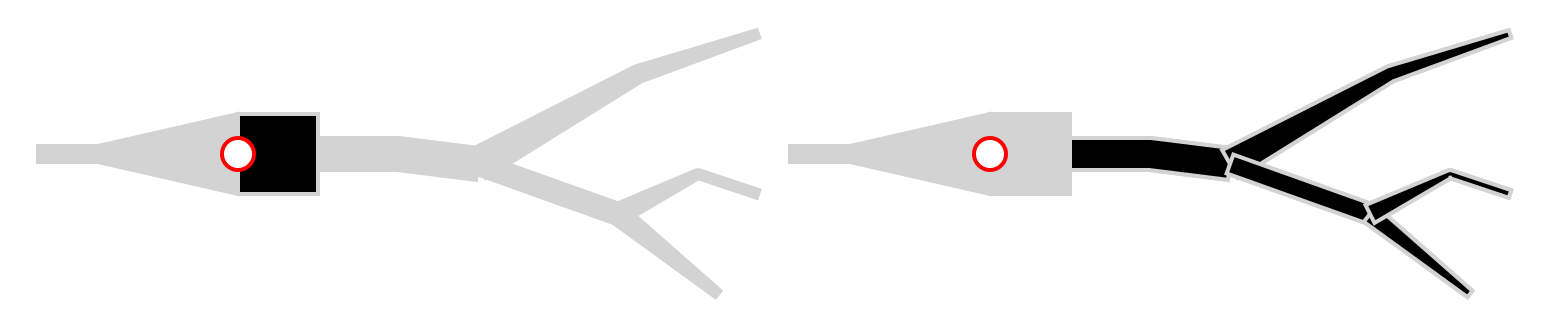
\includegraphics[width=0.6\textwidth]{tag_label}};
          \node at ( 2, 5.5) (l_soma) {Soma};
          \node at ( 5, 5.5) (l_syn) {Synapse};
          \node at (10, 5.5) (l_dend) {Dendrite};
          \node at ( 8, 2) {The Cell};
          \draw[->, ultra thick, black!80, >=stealth] (l_syn.south) to[in=90, out=270] (4.25, 3.75);
        \end{tikzpicture}
    \end{column}
    \begin{column}[T]{0.25\textwidth}
      \textbf{The Network}
      \begin{itemize}
        \item $N$ cells in total, sub-divided into rings of size $n$.
        \item One connection from the soma of cell $i$ to the soma of cell $i + 1 \mod n$
        \item A spike is injected at $t=0$ which will propagate indefinitely through the ring.
        \item A configurable number of additional connections with zero weight
              are added between rings.
        \item These stress the system's interconnect, but do not alter the
              rings' behaviour.
        \item The number of spikes generated on all cells is collected to
              provide a measure of validation.
      \end{itemize}
    \end{column}
  \end{columns}

  \vspace*{1ex}
  \textcolor{arborange}{\rule{\textwidth}{0.5ex}}
  \vspace*{-1ex}
  \begin{columns}[t]
    \begin{column}[T]{0.25\textwidth}
      \textbf{Results}
      \begin{itemize}
        \item We have run this benchmark at varying scales on the JUWELS Booster
        system at the JSC.
        \begin{itemize}
          \item 4 $\times$ A100 GPU per node.
          \item $160\,GB$ of GPU memory.
          \item $40\, TF/s$ of double precision compute.
        \end{itemize}
        \item We chose $d=10$, $n=8$, $p=0.5$, $k=1$, and $l=200\,\mu m$ for the
              parameters.
        \item Single node profiling shows strong dominance of a single ion
              channel with $45\%$ time spent. Requires solving a
              $12\times 12$ linear system per compartment.
        \item Solving the cable equation is the second most relevant cost centre with $15\%$.
        \item The workload is limited by the available GPU memory to around
              $195,000$ cells per node.
        \item (Below) Strong scaling across the GPUs on a single node, showing a
              small degradation in scaling at $1024$ cells per GPU.
        \item (Right) Strong scaling of different cell counts across up to 256
              nodes, efficiency equally falls off at $1024$ cells per GPU.
      \end{itemize}
    \end{column}
    \begin{column}[T]{0.45\textwidth}
      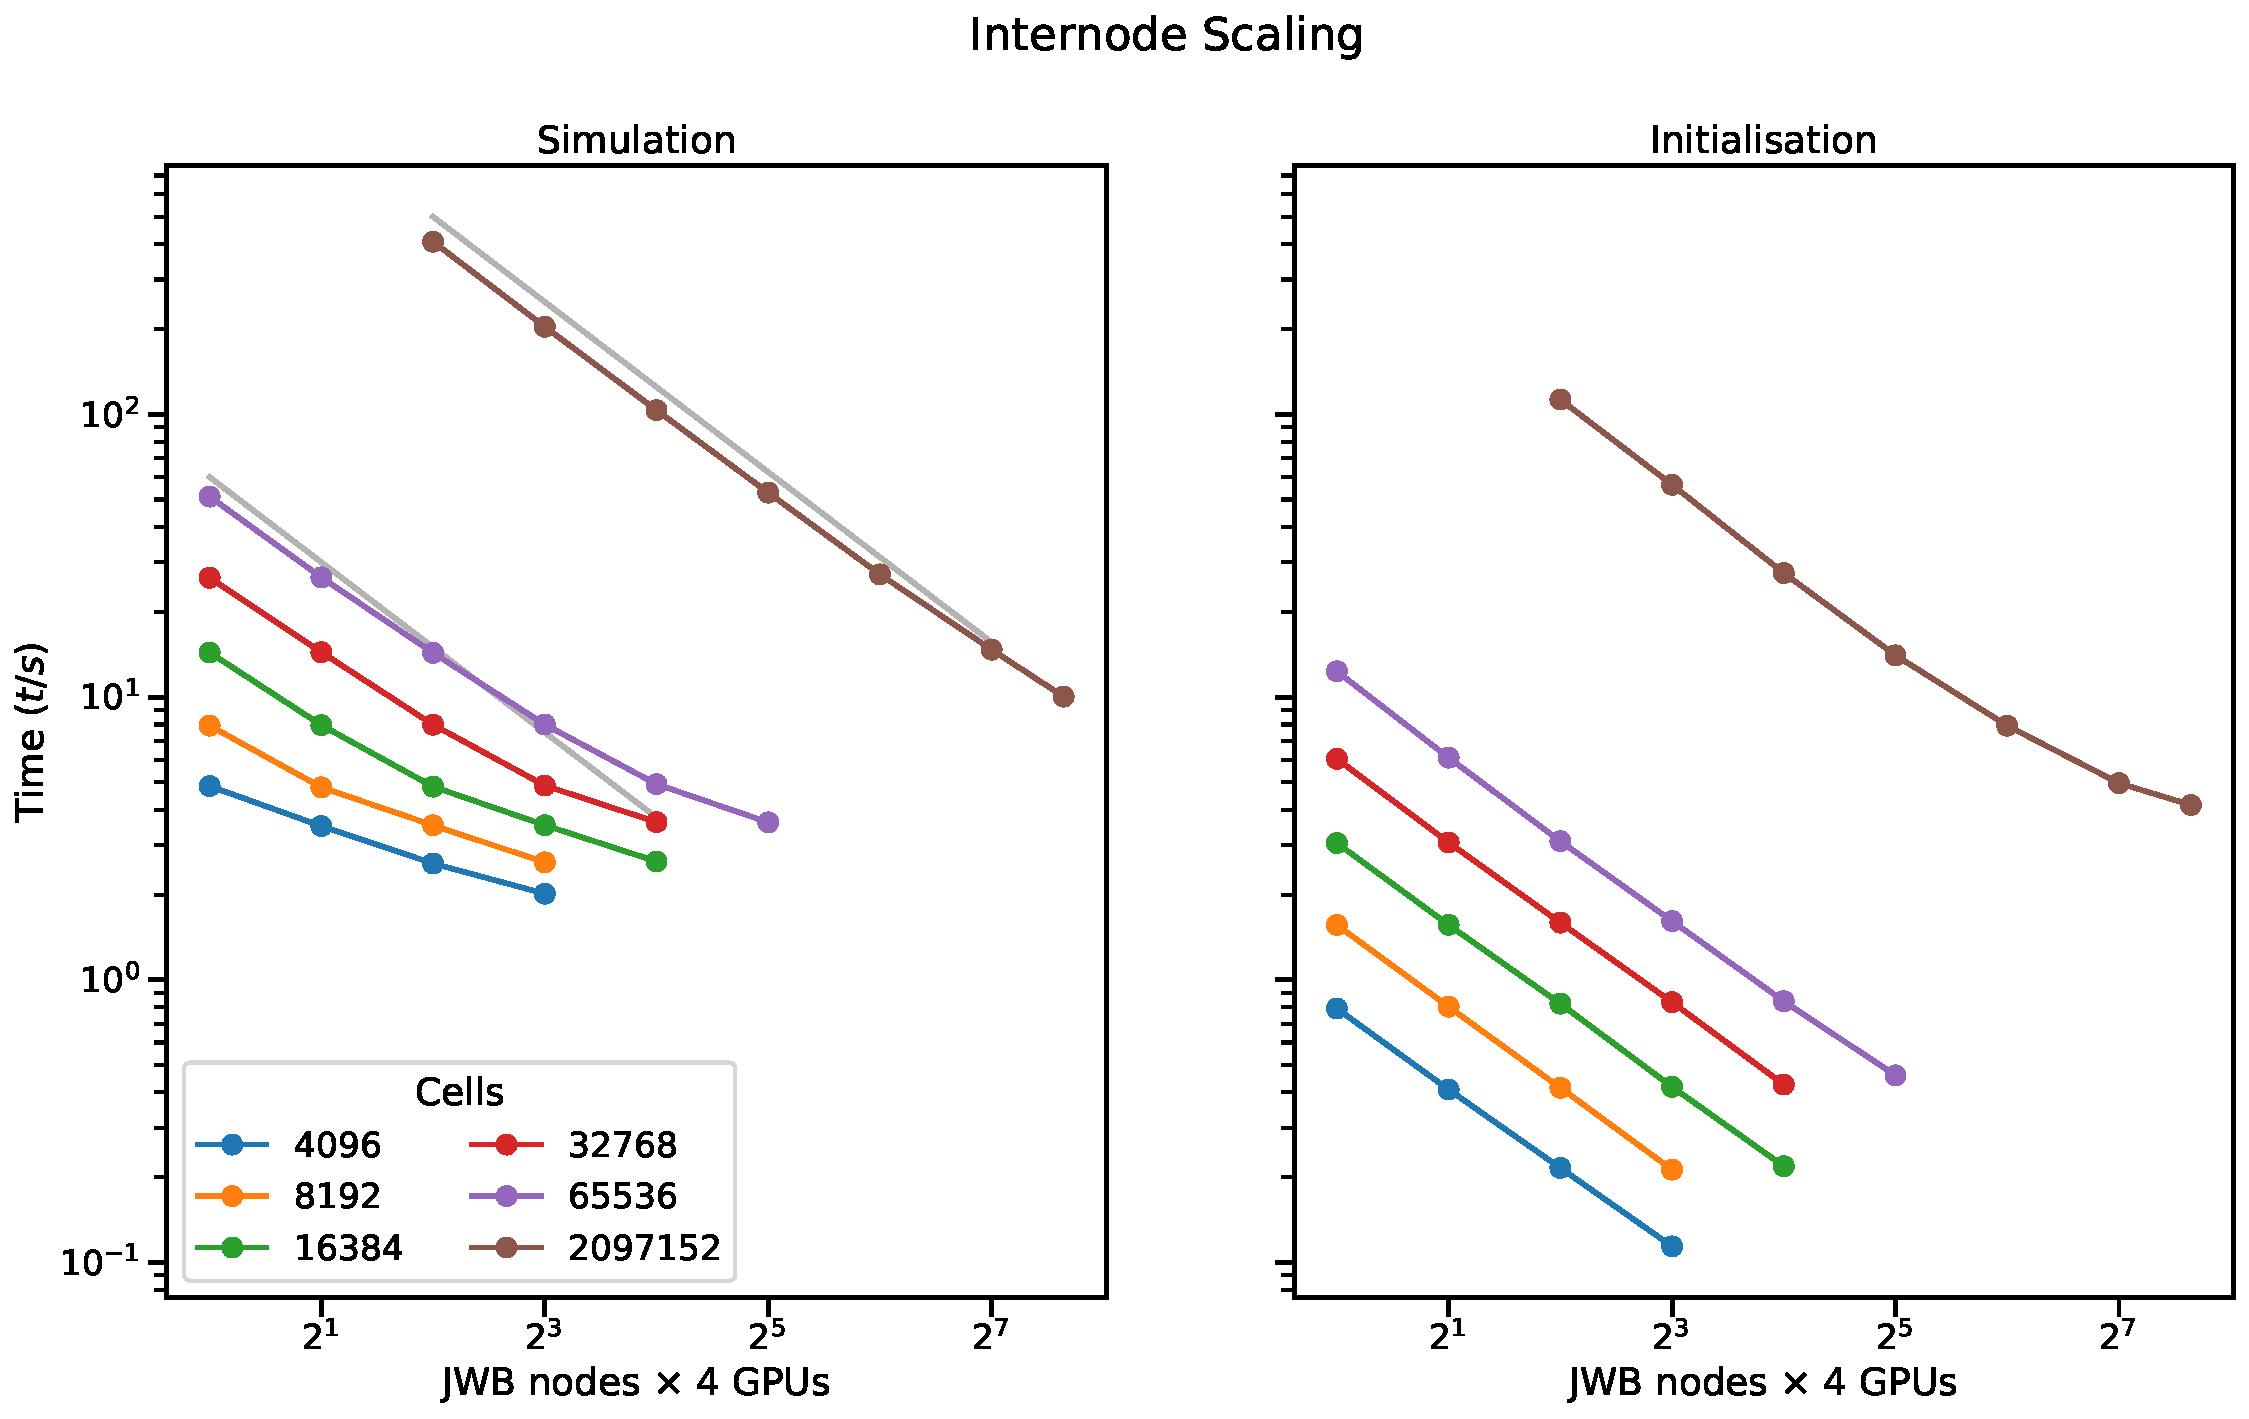
\includegraphics[width=\textwidth]{internode}
    \end{column}
    \begin{column}[T]{0.25\textwidth}
      \textbf{Parallel Efficiency}

      Efficiency $\epsilon$: the ratio of observed to perfect scaling
      \begin{align*}
        \epsilon = \frac{T(n_{0})}{n\cdot T(n)}
      \end{align*}
      For 65536 cells, where $n_{0}= 4$ nodes:
      \begin{center}
        \begin{tabular}{lccc}
          \toprule
          Nodes & $\epsilon_\mathrm{init}$ & $\epsilon_\mathrm{sim}$ & $\epsilon_\mathrm{total}$ \\
          \midrule
          8   & 1.00 & 1.00 & 1.00\\
          16  & 1.03 & 0.99 & 0.99\\
          32  & 1.00 & 0.97 & 0.97\\
          64  & 0.89 & 0.94 & 0.93\\
          128 & 0.71 & 0.87 & 0.83\\
          200 & 0.54 & 0.81 & 0.73\\
          \bottomrule
        \end{tabular}
      \end{center}
      Note that the initialisation time is weighted more heavily in
      $\epsilon_\mathrm{total}$ than one would expect for production use, as the
      simulated biological time in this benchmark is quite short with $200\,ms$.
      Typically, the simulated time is of the order of tens of seconds at least.
    \end{column}
  \end{columns}
  \vspace*{1ex}
  \textcolor{arbgrey}{\rule{\textwidth}{0.5ex}}
  \vspace*{-1ex}
  \begin{columns}[t]
    \begin{column}[T]{0.25\textwidth}
      \textbf{Conclusion}

      Designing a neuro science specific HPC benchmark
      \begin{itemize}
        \item Scalable for approximating relevant neuro science
              workloads on existing and emerging architectures.
        \item Workloads can be tuned to stress a mix of system parameters, i.e.
              computation and interconnect.
        \item In active use to evaluate existing and upcoming systems at the JSC.
        \item Allows for studying the performance characteristics of detailed versus point models.
      \end{itemize}

      Scaling results for Arbor on JUWELS booster.
      \begin{itemize}
        \item For the showcased workload, Arbor shows scaling up to $256$ nodes on
              JUWELS booster with above $80\%$ efficiency.
        \item Below $1000$ cells per GPU efficiency falls off; indicating the
              limit of strong scaling.
        \item Identified some potential areas for improving scalability and
              overall performance of Arbor.
      \end{itemize}
    \end{column}

    \begin{column}[T]{0.45\textwidth}
      \centering
      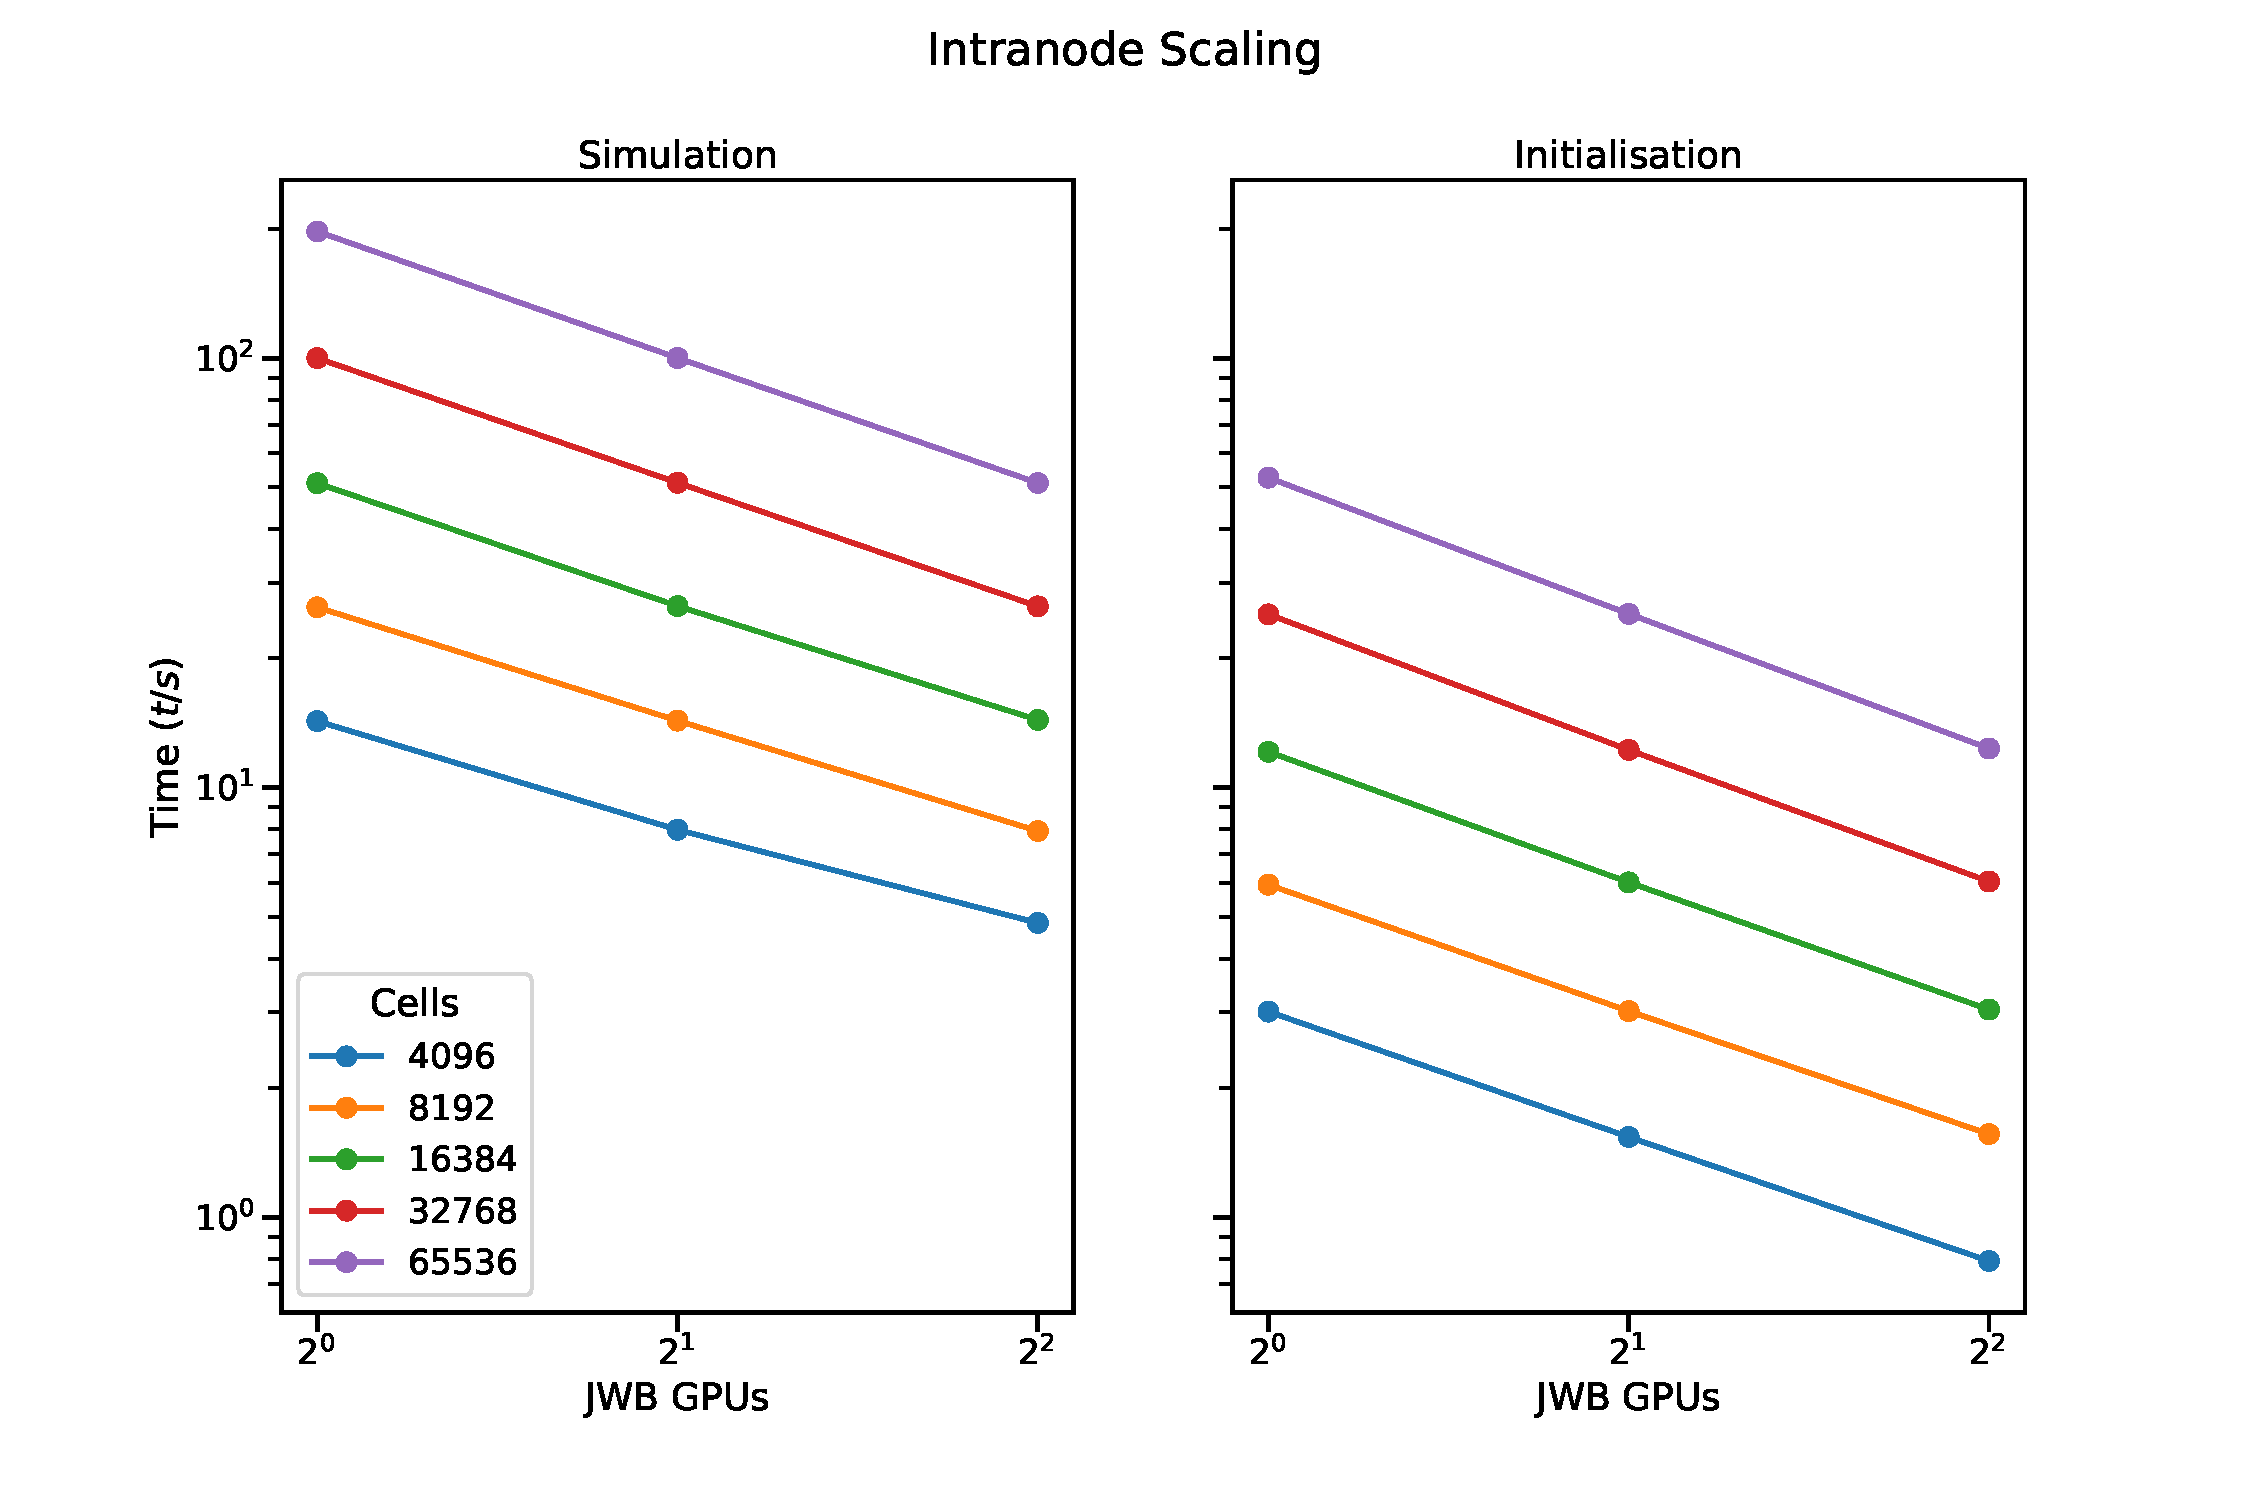
\includegraphics[width=0.9\textwidth]{intranode}
    \end{column}
    \begin{column}[T]{0.25\textwidth}
      \textbf{Future Work}

      \begin{itemize}
        \item Extend the node counts to the full JUWELS booster of up to 936
              nodes.
        \item Performing deeper performance analysis of the code under this
              specific workload.
        \item We identified a series of potential improvements to Arbor
           \begin{itemize}
             \item The linear solver used in the ion channels.
             \item Arguments to GPU kernels are packed into a single
                   struct, which could lead to performance problems.
             \item The DSL compiler for GPU kernels might be improved.
             \item Reducing the amount of host/device data transfer.
             \item Reducing the memory overhead per cell.
           \end{itemize}
        \item We plan to evaluate the AMD Instinct and NVIDIA Hopper
              architectures, as soon as they become available to us. This is both
              to evaluate these novel designs and to further the development of
              Arbor.
        \item Investigate a mixed workload consisting of point neurons located
              on the CPU and complex models driven by the GPU of the node.
      \end{itemize}
    \end{column}
  \end{columns}

  \vspace*{1ex}
  \textcolor{arbred}{\rule{\textwidth}{0.5ex}}
  \vspace*{-1ex}
  \begin{columns}
    \begin{column}[T]{0.49\textwidth}
      \textbf{References}
      \printbibliography
    \end{column}
    \begin{column}[T]{0.49\textwidth}
      \textbf{Acknowledgements}

      This research has received funding from the European Union's Horizon 2020
      Framework Programme for Research and Innovation under the Specific Grant
      Agreements No.\,720270 (HBP SGA1), No.\,785907 (HBP SGA2), and No.\,945539
      (HBP SGA3).
    \end{column}
  \end{columns}
\end{frame}
\end{document}
